% Fig. 1, evaluation framework. Compiled by paper/build.py to Figure1.pdf and Figure1.png (600 dpi).
\documentclass[border=2pt]{standalone}
\usepackage[T1]{fontenc}
\usepackage{mathptmx}
\usepackage{tikz}
\usetikzlibrary{positioning,arrows.meta,fit,calc}
\definecolor{ink}{HTML}{1F2937}
\definecolor{dataC}{HTML}{E8F1FB}
\definecolor{trainC}{HTML}{EAF6EC}
\definecolor{auditC}{HTML}{FDF0E6}
\definecolor{xaiC}{HTML}{F1ECFA}
\begin{document}
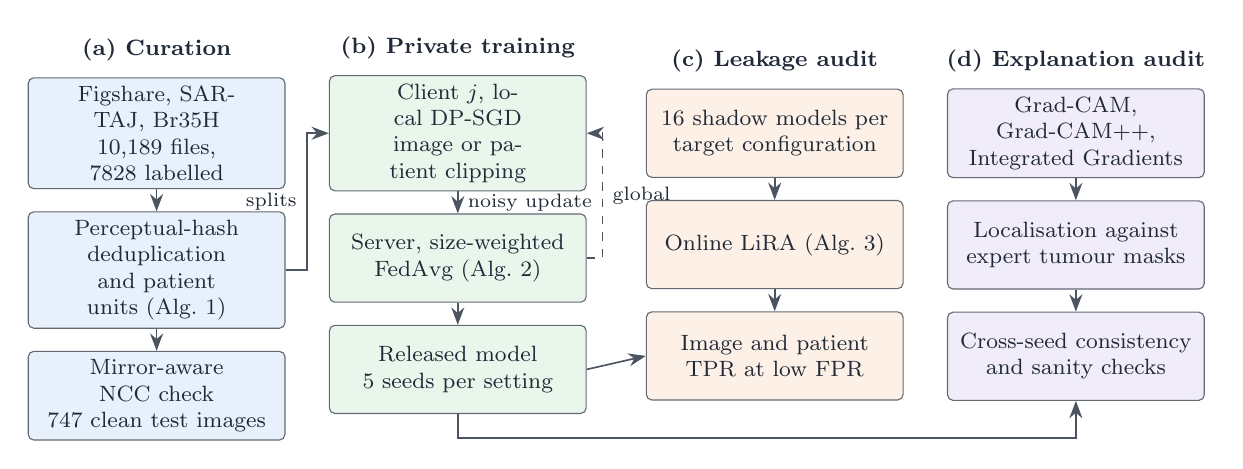
\begin{tikzpicture}[
  font=\footnotesize, text=ink, >={Stealth[length=2.2mm]},
  box/.style={draw=ink!70, rounded corners=2pt, align=center, inner sep=3pt, text width=3.05cm, minimum height=1.12cm},
  stage/.style={font=\footnotesize\bfseries, anchor=south},
  arr/.style={->, draw=ink!80, line width=0.6pt}]
% stage 1 data
\node[box, fill=dataC] (src) {Figshare, SARTAJ, Br35H\\10,189 files, 7828 labelled};
\node[box, fill=dataC, below=0.28cm of src] (dedup) {Perceptual-hash deduplication\\and patient units (Alg.~1)};
\node[box, fill=dataC, below=0.28cm of dedup] (ncc) {Mirror-aware NCC check\\747 clean test images};
\node[stage] at ($(src.north)+(0,0.08)$) {(a) Curation};
% stage 2 training
\node[box, fill=trainC, right=0.55cm of src] (cl) {Client $j$, local DP-SGD\\image or patient clipping};
\node[box, fill=trainC, below=0.28cm of cl] (agg) {Server, size-weighted\\FedAvg (Alg.~2)};
\node[box, fill=trainC, below=0.28cm of agg] (model) {Released model\\5 seeds per setting};
\node[stage] at ($(cl.north)+(0,0.08)$) {(b) Private training};
% stage 3 audit
\node[box, fill=auditC, right=0.75cm of cl] (sh) {16 shadow models per\\target configuration};
\node[box, fill=auditC, below=0.28cm of sh] (lira) {Online LiRA (Alg.~3)};
\node[box, fill=auditC, below=0.28cm of lira] (mia) {Image and patient\\TPR at low FPR};
\node[stage] at ($(sh.north)+(0,0.08)$) {(c) Leakage audit};
% stage 4 explanations
\node[box, fill=xaiC, right=0.55cm of sh] (cam) {Grad-CAM, Grad-CAM++,\\Integrated Gradients};
\node[box, fill=xaiC, below=0.28cm of cam] (loc) {Localisation against\\expert tumour masks};
\node[box, fill=xaiC, below=0.28cm of loc] (cons) {Cross-seed consistency\\and sanity checks};
\node[stage] at ($(cam.north)+(0,0.08)$) {(d) Explanation audit};
% arrows
\draw[arr] (src) -- (dedup);
\draw[arr] (dedup) -- (ncc);
\draw[arr] (cl) -- node[right, font=\scriptsize]{noisy update} (agg);
\draw[arr] (agg) -- (model);
\draw[arr, dashed] (agg.east) -- ++(0.2,0) |- node[pos=0.25, right, font=\scriptsize]{global} (cl.east);
\draw[arr] (sh) -- (lira);
\draw[arr] (lira) -- (mia);
\draw[arr] (cam) -- (loc);
\draw[arr] (loc) -- (cons);
\draw[arr] (dedup.east) -- ++(0.27,0) |- node[pos=0.25, left, font=\scriptsize]{splits} (cl.west);
\draw[arr] (model.east) -- (mia.west);
\draw[arr] (model.south) -- ++(0,-0.3) -| (cons.south);
\end{tikzpicture}
\end{document}
